\documentclass[10pt, a4paper]{report}

%used packages
% To indent first paragraph in article
\usepackage[]{indentfirst}
%To make multicolumn list
\usepackage{multicol}
%To use graphics
\usepackage{graphicx}
%To make figures side by side
\usepackage{caption}
\usepackage{subcaption}
%To include urls
%\usepackage{hyperref}
\usepackage[margin = 1.7in]{geometry}
\graphicspath{{graphs/}}


\author{Mahmoud Agha}
\title{Pharmacokinetic Properties of Chlordiazepoxide, diazepam ,and lorazepam (Benzodiazepines)}

\begin{document}
\maketitle
\tableofcontents
	\begin{abstract}
		Benzodiazepines are a class of psychoactive drugs that interact with the \emph{GABA$_A$} receptors. They consist of a typical structure of benzene ring attached to a diazepine ring. The different drugs differ in the substituents that are attached to the benzodiazepine core. We summarize the properties of three of drugs of the benzodiazepine  family: Chlordiazepoxide, diazepam ,and lorazepam. We report on their discovery, mechanism of action, site of action, pharmacokinetic properties, metabolites, active metabolites, side-effects, toxicity, as well as dosage forms. 
	\end{abstract}

%Pharmacological Class
\chapter{Pharmacological Class}
The three drugs Chlordiazepoxide, diazepam, and lorazepam belong to a class of drugs named benzodiazepines\footnote{BZD, BZs or benzos}

\section{Chemical Structure}
Benzodiazepines consist of a benzene ring attached to diazepine ring.
The chlordiazepoxide has an (N-methylamine) substitued on position 2, an oxygen on position $4$, and a chlorine atom on postion 7 on the benzodiazepine.
Diazepam has a methyl group on position 1, an oxygen on position 2, and a chlorine on position 7.
Lorazepam has an oxygen on position 2, a hydroxyl on position 3, a chlorine on position $2'$.

Benzodiazepines are a class of psychoactive drugs. that enhance the effect of \emph{\uppercase{gaba}} at the \emph{GABA$_A$} receptor which results in sedative, hypnotic, anxiolytic, anticonvulsant, muscle relaxant properties.

Benzodiazepines are used in treating anxiety, insomnia, agitation, sezures, mmuscle spasms, alcohol withdrawal.\cite{}

%discovery
\input{./parts/disc.tex}
%Mecahnism of Action done
\chapter{Mechanism of Action}
Benzodiazepines induce a calming effect by increasing the efficiency of a natural brain chemical\emph{GABA} which leads to a decrease in the excitability of neurons.

GABA$_A$ receptors are heteropentameric membrane proteins that form a chloride channel. They are composed of several subunits ($\alpha 1-6, \beta 1-3, \gamma 1-3, \delta, \epsilon, \theta, \pi$, and $\rho 1-4$). The \emph{GABA} receptors are sensitive to benzodiazepines specifically those that contain the $\alpha(1,2,3,5)$, $\beta(2,3)$ and $\gamma 2$ subunits in a $2:2:1$ stoichiometry.

\emph{GABA} binds to the \emph{GABA$_A$} receptors and open the chloride channels and causes a change in potential of the membrane. Benzodiazepines interact allosterically with the \emph{GABA$_A$} and increase the affinity of \emph{GABA} to the \emph{GABA$_A$} receptors. The change at the molecular level is that when benzodiazepines bind to the \emph{GABA$_A$} receptors they prolong the duration at which the \emph{GABA} binds to the its receptor and thus increase the amount of charge that being transferred, this leads to an increase in potential across the membrane of the cell.


The \emph{GABA} itself which is the main drug that induces the action activate the \emph{GABA$_A$} receptor which upon activation conducts chloride ions selectively across the membrane which results in hyperpolarization thus inhibiting the neurotransmission by reducing the potential of having an action-potential. 

Benzodiazepine stimulate the sedative effect by acting on the \emph{GABA$_A-\alpha 1$} receptor\cite{rudolph1999benzodiazepine} and stimulate anxiolytic\footnote{anti-anxiety} by interacting with the \emph{GABA$_A-\alpha 2$} receptor.\cite{kopp2004modulation} 





%Site of Action done
%\chapter{Site of Action}
Benzodiazepines act on the \emph{GABA$_A$} which are present in the central nervous system. The distribution and types of \emph{GABA$_A$} vary widely between regions and subtypes of the \emph{GABA$_A$} receptors are repsonsible for different actions including anxiolytic, and hyponitic activity.

%Pharmacokintics done
\chapter{Pharmacokinetics}

\section{Chlordiazepoxide}
%Draw chemical structure of the metabolites in the metabolites section
The complexity of chlordiazepoxide arise from the pharmacologically actie metabolites that it gets transformed into such as desmethylchlordiazepoxide, demoxepam, desmethyldiazepam, and oxazepam.\footnote{The chemical structures are to be found in the metabolites chapter \ref{sec:met:chlor}}

The elimination half-life (t$\frac{1}{2}\beta$) of single doses of chlordiazepoxide in healthy individuals ranges from from $5$ to $30$ hours, the volume of distrubtion ($V_d$) ranges from $0.25$ to $0.50$ liters/kg. The hepatic extraction ratio is under $5\%$.

Clearance of chlordiazepoxide is reduced in the elderly, patients with cirrhosis\footnote{an abnormal liver condition in which there is irreversible scarring of the liver.}, and patients receiving concurrent medicationof disulfiram\footnote{known as Antabus and is used in treatment of alcoholism}. Oral doses are absorbed completely and rapidly, while intramuscular injection is painful and results in slow unpredictable absorption.\cite{Greenblatt1978}  

\section{Diazepam}
\subsection{Absorption}
Oral bioavailibity of diazepam is about $0.9$ and the average time to achieve a peak in plasma concentration (T$_{max}$) ranges from 1 to $1.5$ hours. High fat food increases increases absorption lag time to about $45$ minutes as compared with $15$ minutes for a fasting person, and an increase in T$_{max}$ to about $2.5$ hours. C$_{max}$ also drops by $20\%$ and AUC drops by about $27\%$ (range $15\%$ to $50\%$).

\subsection{Distribution}
Diazepam along with its metabolites show high affinity to plasma proteins ($98\%$). Diazepam along with its metabolites have a high lipophilicity and thus cross the blood-brain barrier along with the placenta, and is found in breast milk in concentrations of about $\frac{1}{10}$ of the maternal plasma.
The volume of distribution (V$_d$) at steady state is about $0.8$ to $1.0$ L/kg. Diazepam shows a biphasic plasma concentration-time profile after oral administration. The  distribution phase has a half-life of about $1$ to $>3$hours.

\subsection{Metabolism}
Diazepam tranforms to nordiazepam (gets N-methylated) by [Cytochrome P450 2C9, Cytochrome P450 2B6, Cytochrome P450 2C19, Cytochrome P450 3A5, Cytochrome P450 3A4],\cite{zhou2009substrates} gets metabolized to temazepam by [Prostaglandin G/H synthase 1, Cytochrome P450 2C19], and to oxazepam by cytochrome P$450$ $1$A$2$, it also gets metabolized to desmehtyldiazepam.

Noridazepam gets metabolized to oxazepam by [Cytochrome P450 2C19, Cytochrome P450 3A4, Cytochrome P450 3A5], it also gets metabolized to Nordiazepam O-glucuronide.

Tamazepam gets metabolized to Oxazepam by [Cytochrome P450 2B6, Cytochrome P450 2C9, Cytochrome P450 2C19, Cytochrome P450 3A4, Cytochrome P450 3A5]

\subsection{Elimination}
The elimination phase following the distribution phase has a half-life of about $48$ hours. The eliminatino half-life time of the active metabolite N-desmethyldiazepam is up to $100$ hours. Diazepams along with its metabolites are excreted in the urine as their glucuronide conjugates. The clearance of diazepam is $20$ to $30$ mL/min. 

\section{Lorazepam}
Lorazepam as a 3-hydroxy benzodiazepine derivative has a major metabolic pathway that involes conjugation to glucuronic acid at position 3. The glucuronide metabolite is inactie and is followed by urinary excretion.

Elimination half-life time ranges between 5 and 15 hours in healthy individuals. The volume of distribution (V$_d$) ranges between 0.6 to 2.0 L/kg which indicates a very high affinity to plasma proteins. Clearance is from $0.9$ to $2.0$ ml/min/kg. Aging and liver diseases do not have a substantial influence on the kinetics of lorazepam, while relan diseases are associated with prolonged half-life and increased volume of distribution.\cite{Greenblatt1981}

%Metabolites needs chemical structure
\chapter{Metabolites}

\section{Chlordiazepoxide}
\label{sec:met:chlor}
The metabolites of chlordiazepoxide are desmethylchlordiazepoxide \emph{Fig} \ref{fig:desmeth}, demoxepam \emph{Fig} \ref{fig:demoxepam}, desmethyldiazepam \emph{Fig} \ref{fig:desmethyldiazepam}, and oxazepam \emph{Fig} \ref{fig:oxazepam}.\cite{schwartz1971biological}

\begin{figure}[h]
	\centering
	\begin{minipage}{0.5\linewidth}
		\centering
		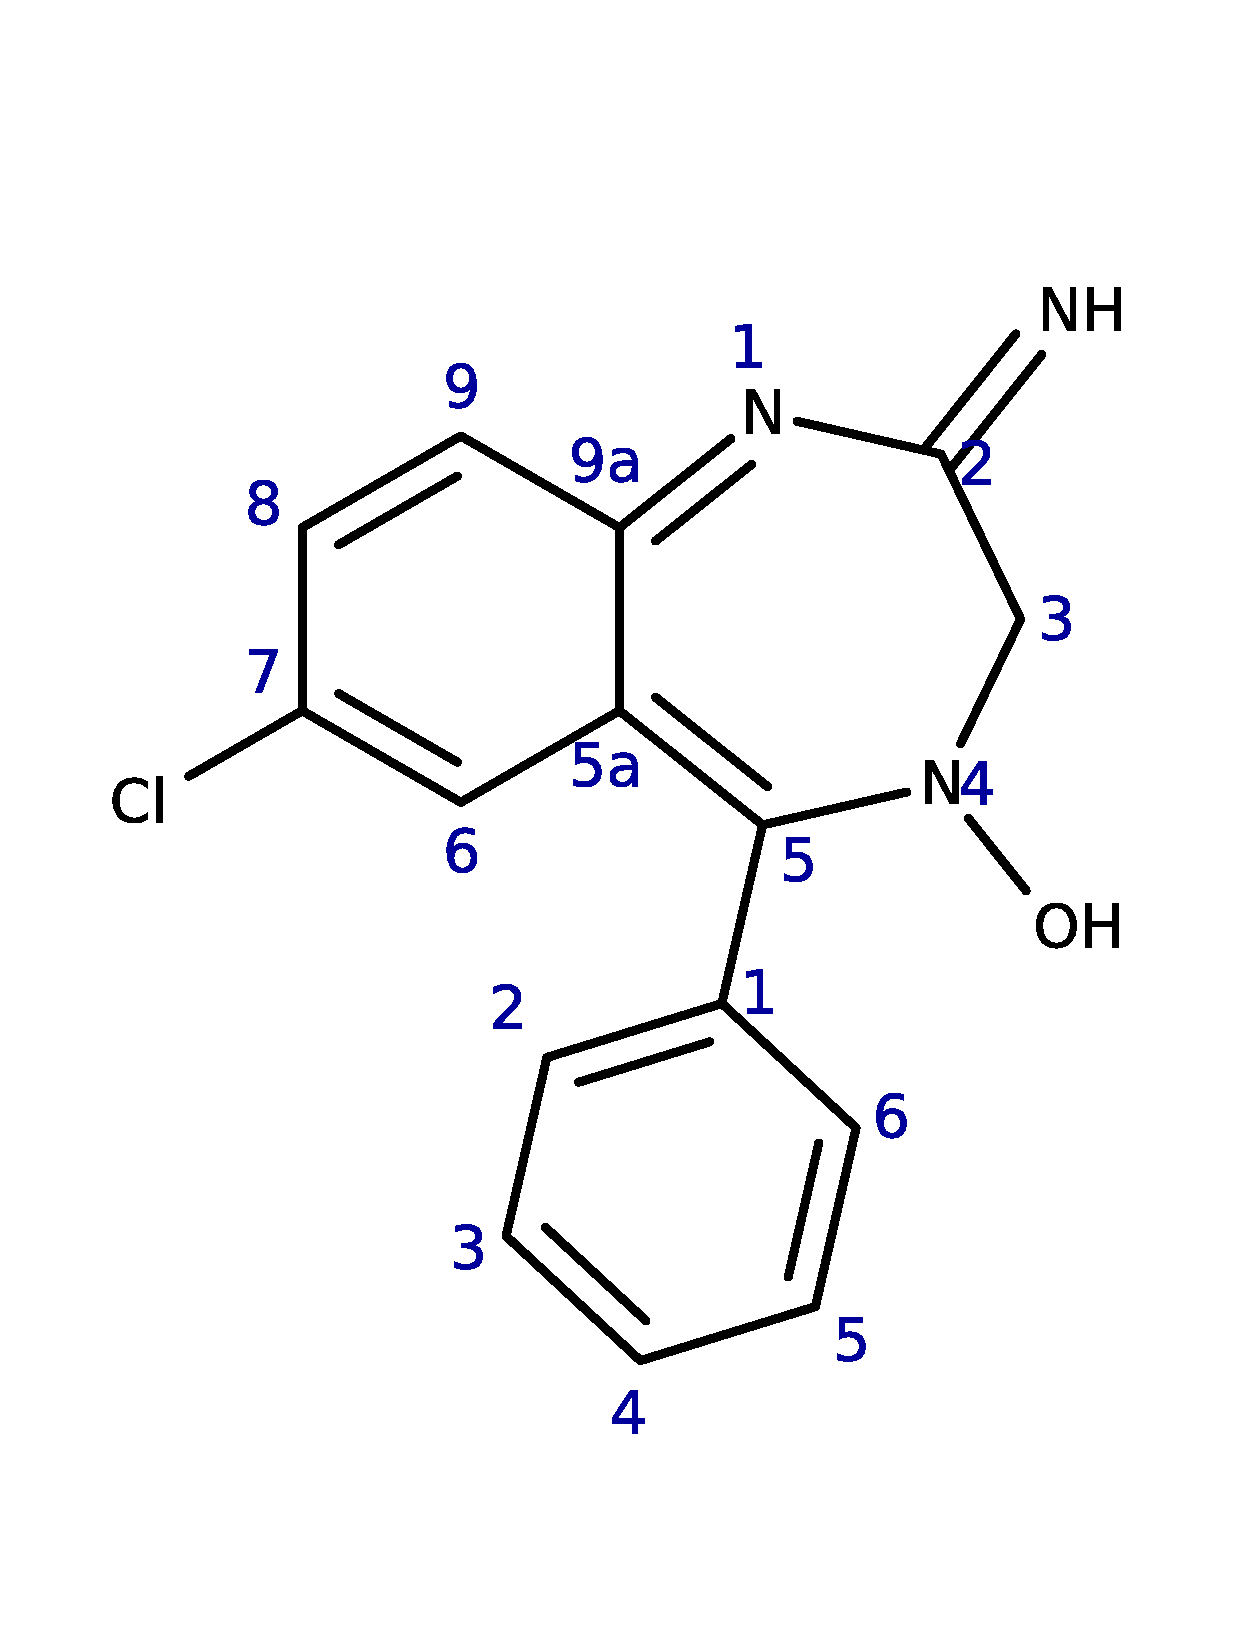
\includegraphics[width=\linewidth]{DesmethylChlordiazepoxide.pdf}
		\captionof{figure}{Desmethylchloridiazepoxide}
		\label{fig:desmeth}
	\end{minipage}%
	\begin{minipage}{0.5\textwidth}
		\centering
		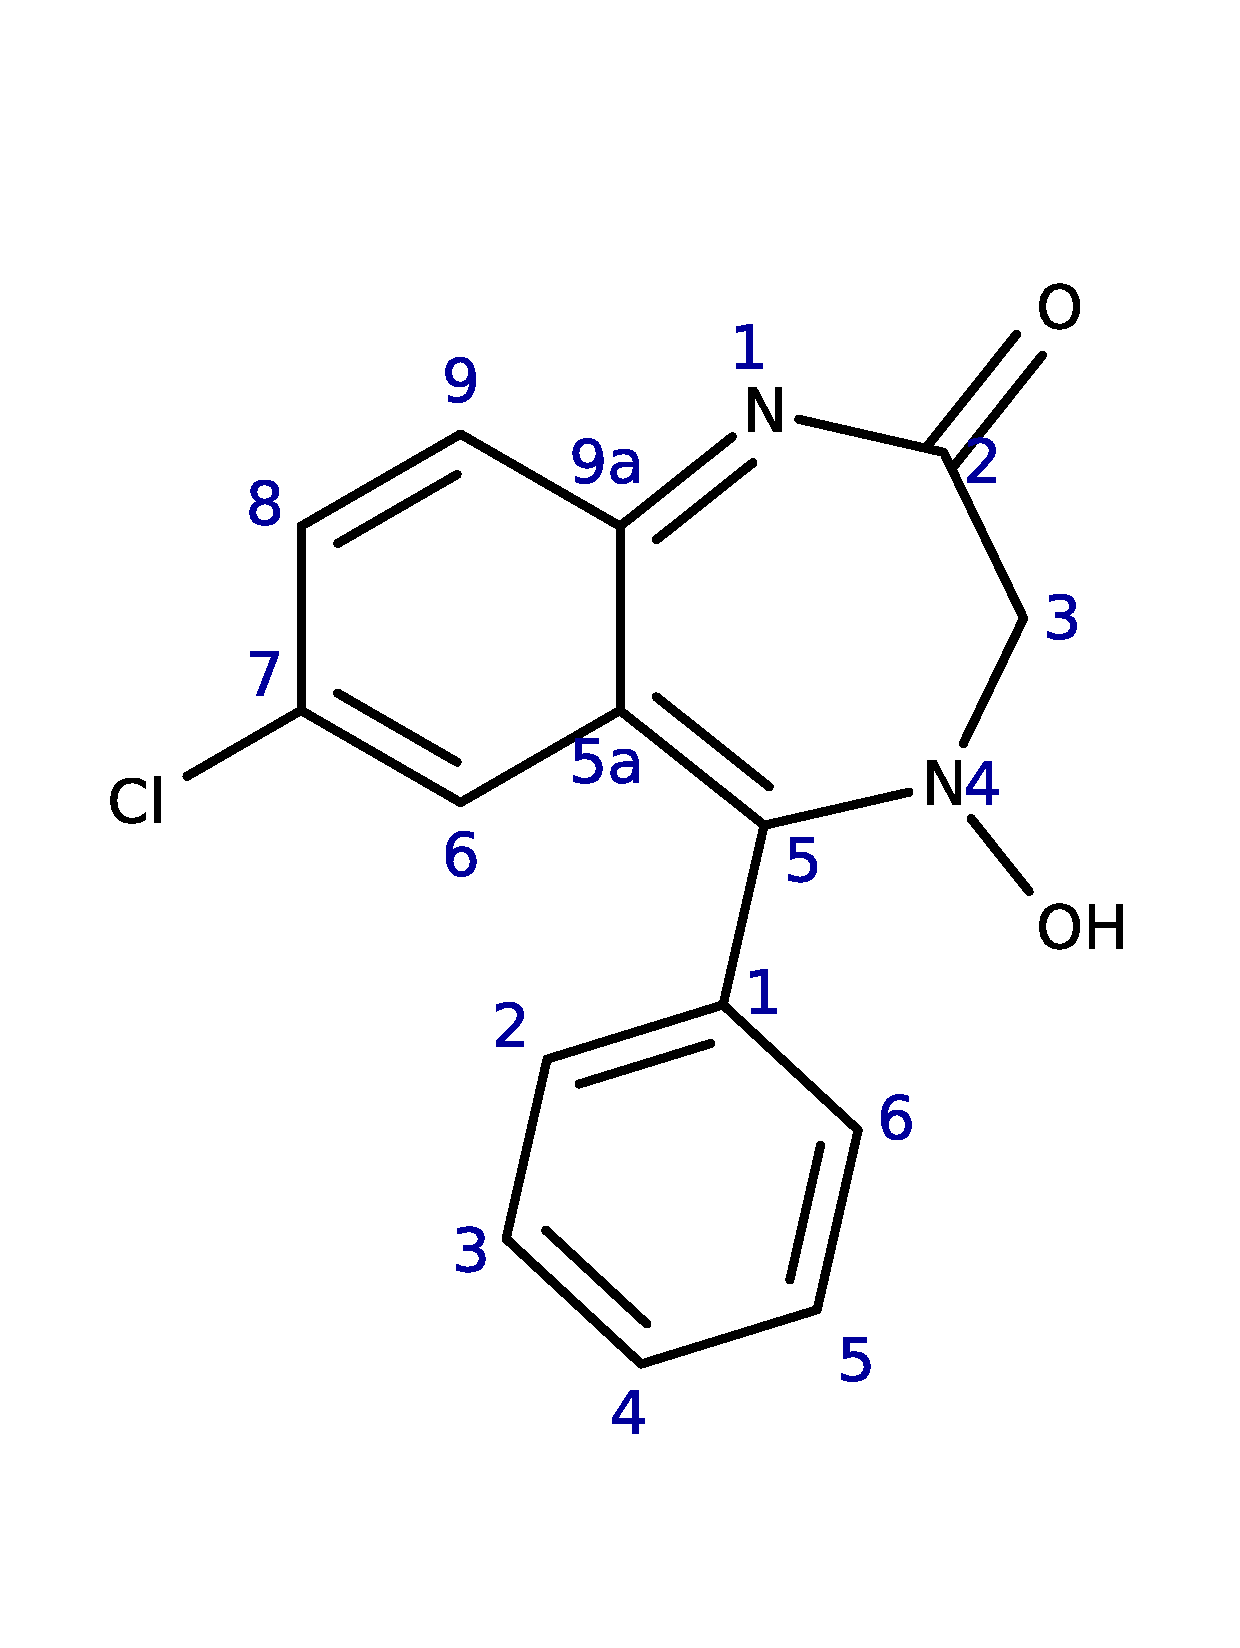
\includegraphics[width=\linewidth]{Demoxepam.pdf}
		\captionof{figure}{Demoxepam}
		\label{fig:demoxepam}
	\end{minipage}
\end{figure}

\begin{figure}[h]
	\centering
	\begin{minipage}{0.5\linewidth}
		\centering
		\includegraphics[width=\linewidth]{desmethyldiazepam.pdf}
		\captionof{figure}{Desmethyldeiazepam}
		\label{fig:desmethyldiazepam}
	\end{minipage}%
	\begin{minipage}{0.5\textwidth}
		\centering
		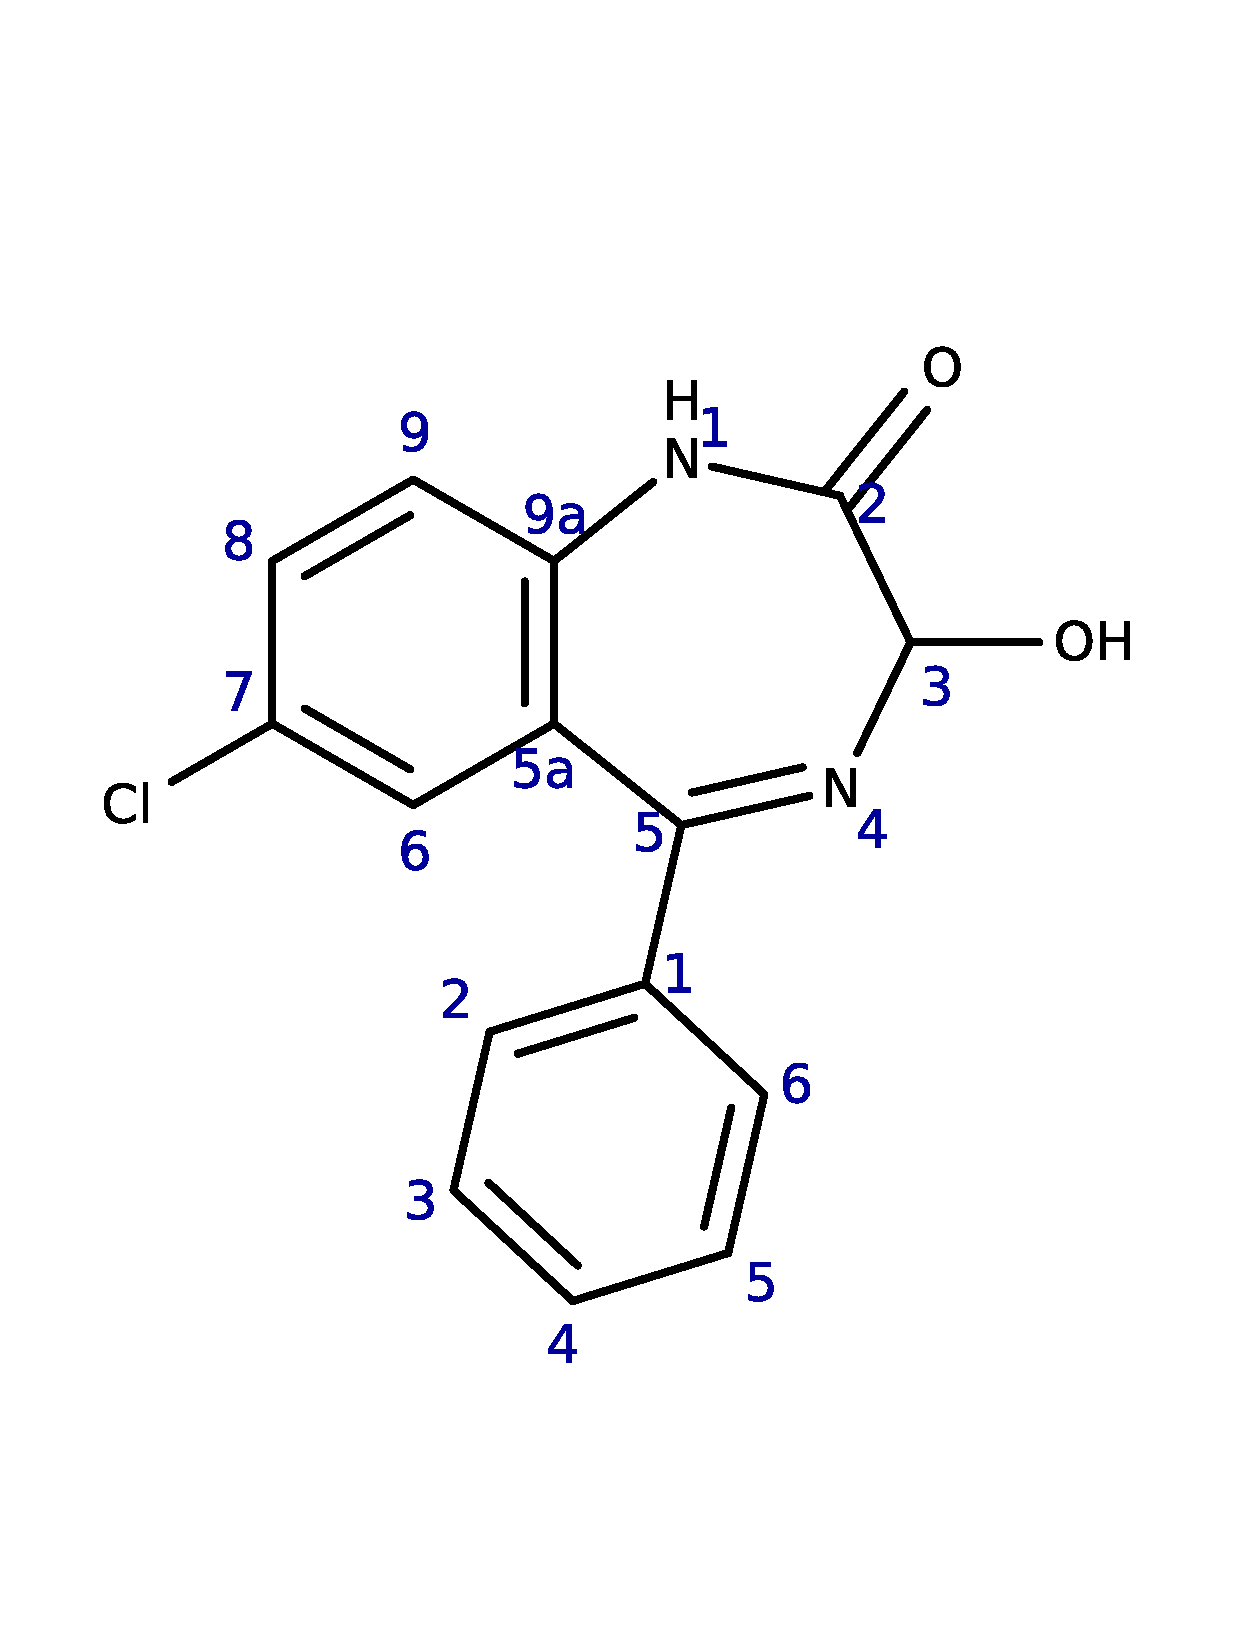
\includegraphics[width=\linewidth]{oxazepam.pdf}
		\captionof{figure}{Oxazepam}
		\label{fig:oxazepam}
	\end{minipage}
\end{figure}


\section{Diazepam}
 	The main active metabolite is desmethyldiazepam \emph{Fig} \ref{fig:desmethyldiazepam}, Along with inactive metabolites like temazepam \emph{Fig} \ref{fig:temazepam}, oxazepam \emph{Fig} \ref{fig:oxazepam}, and Nordiazepam O-glucuronide \emph{Fig} \ref{fig:norgluc}.\cite{RCM:RCM3613}

\begin{figure}[h]
	\centering
	\begin{minipage}{0.5\linewidth}
		\centering
		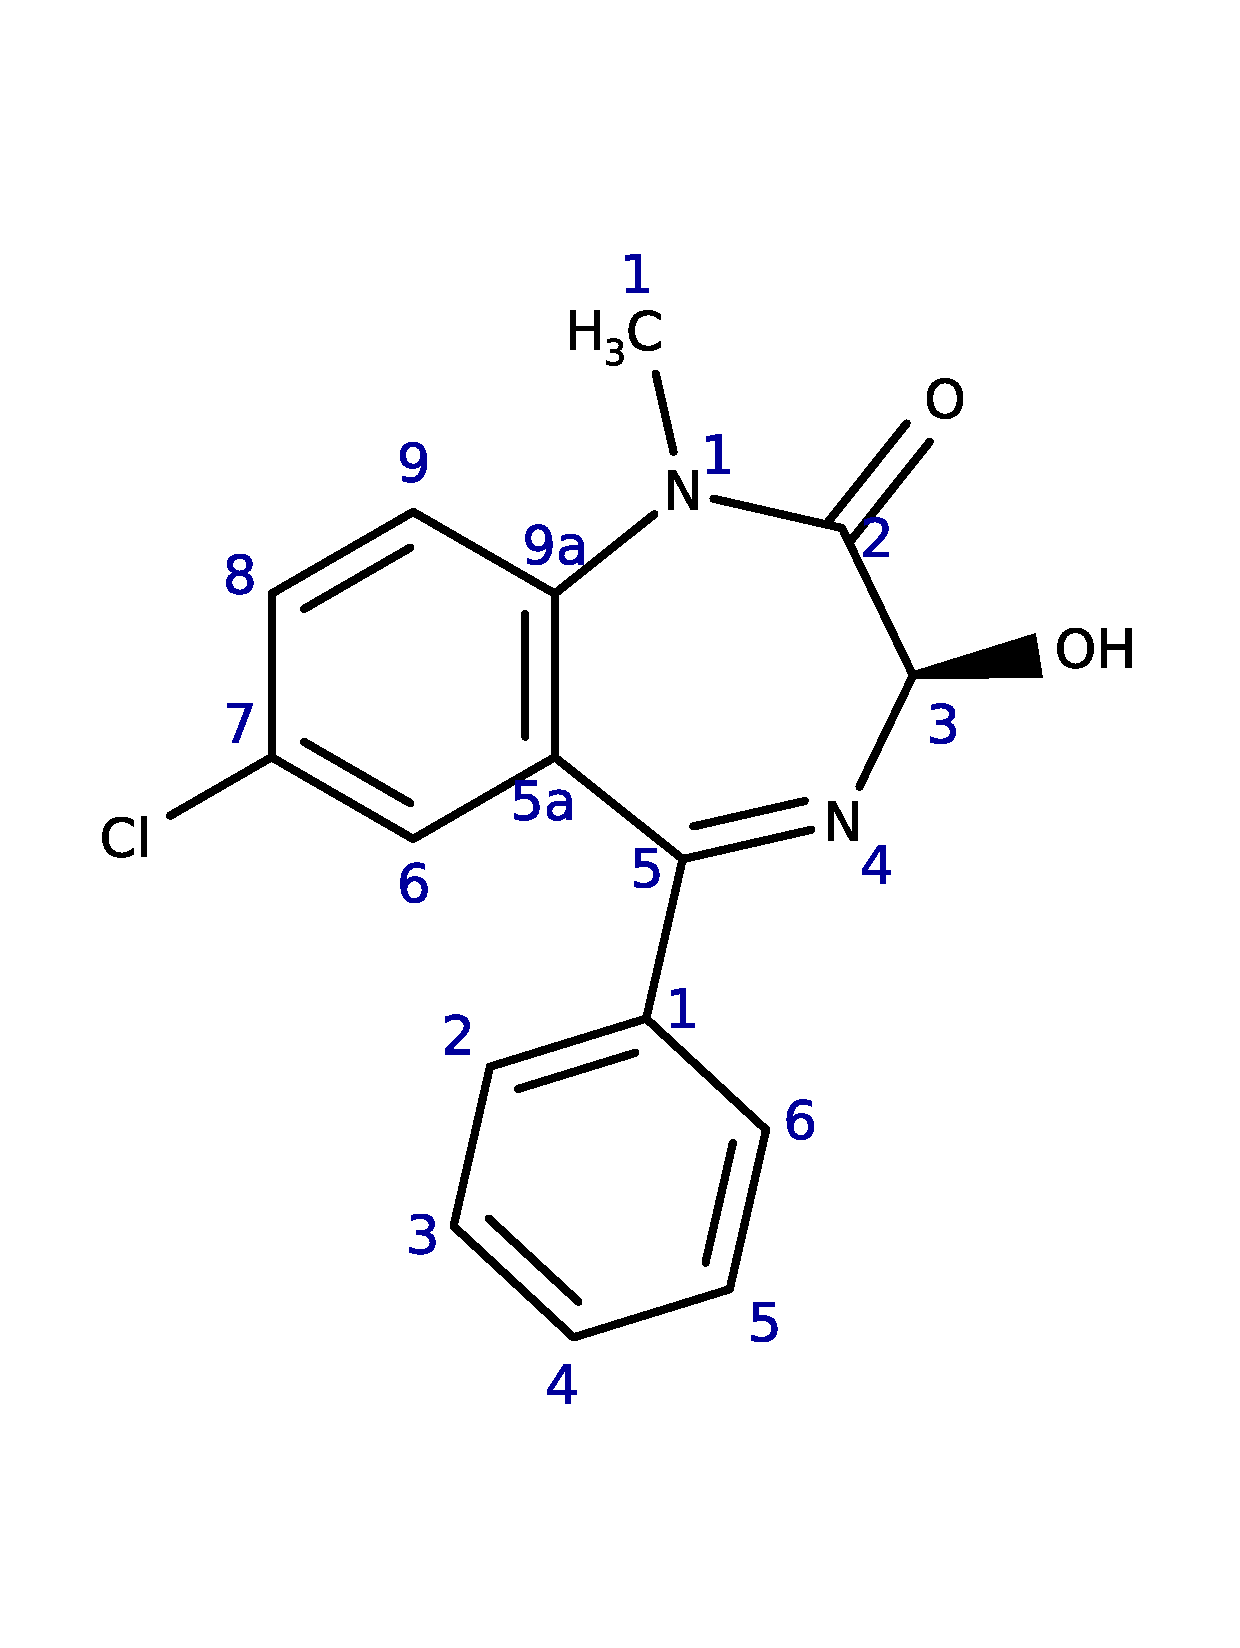
\includegraphics[width=\linewidth]{Temazepam.pdf}
		\captionof{figure}{Temazepam}
		\label{fig:temazepam}
	\end{minipage}%
	\begin{minipage}{0.5\textwidth}
		\centering
		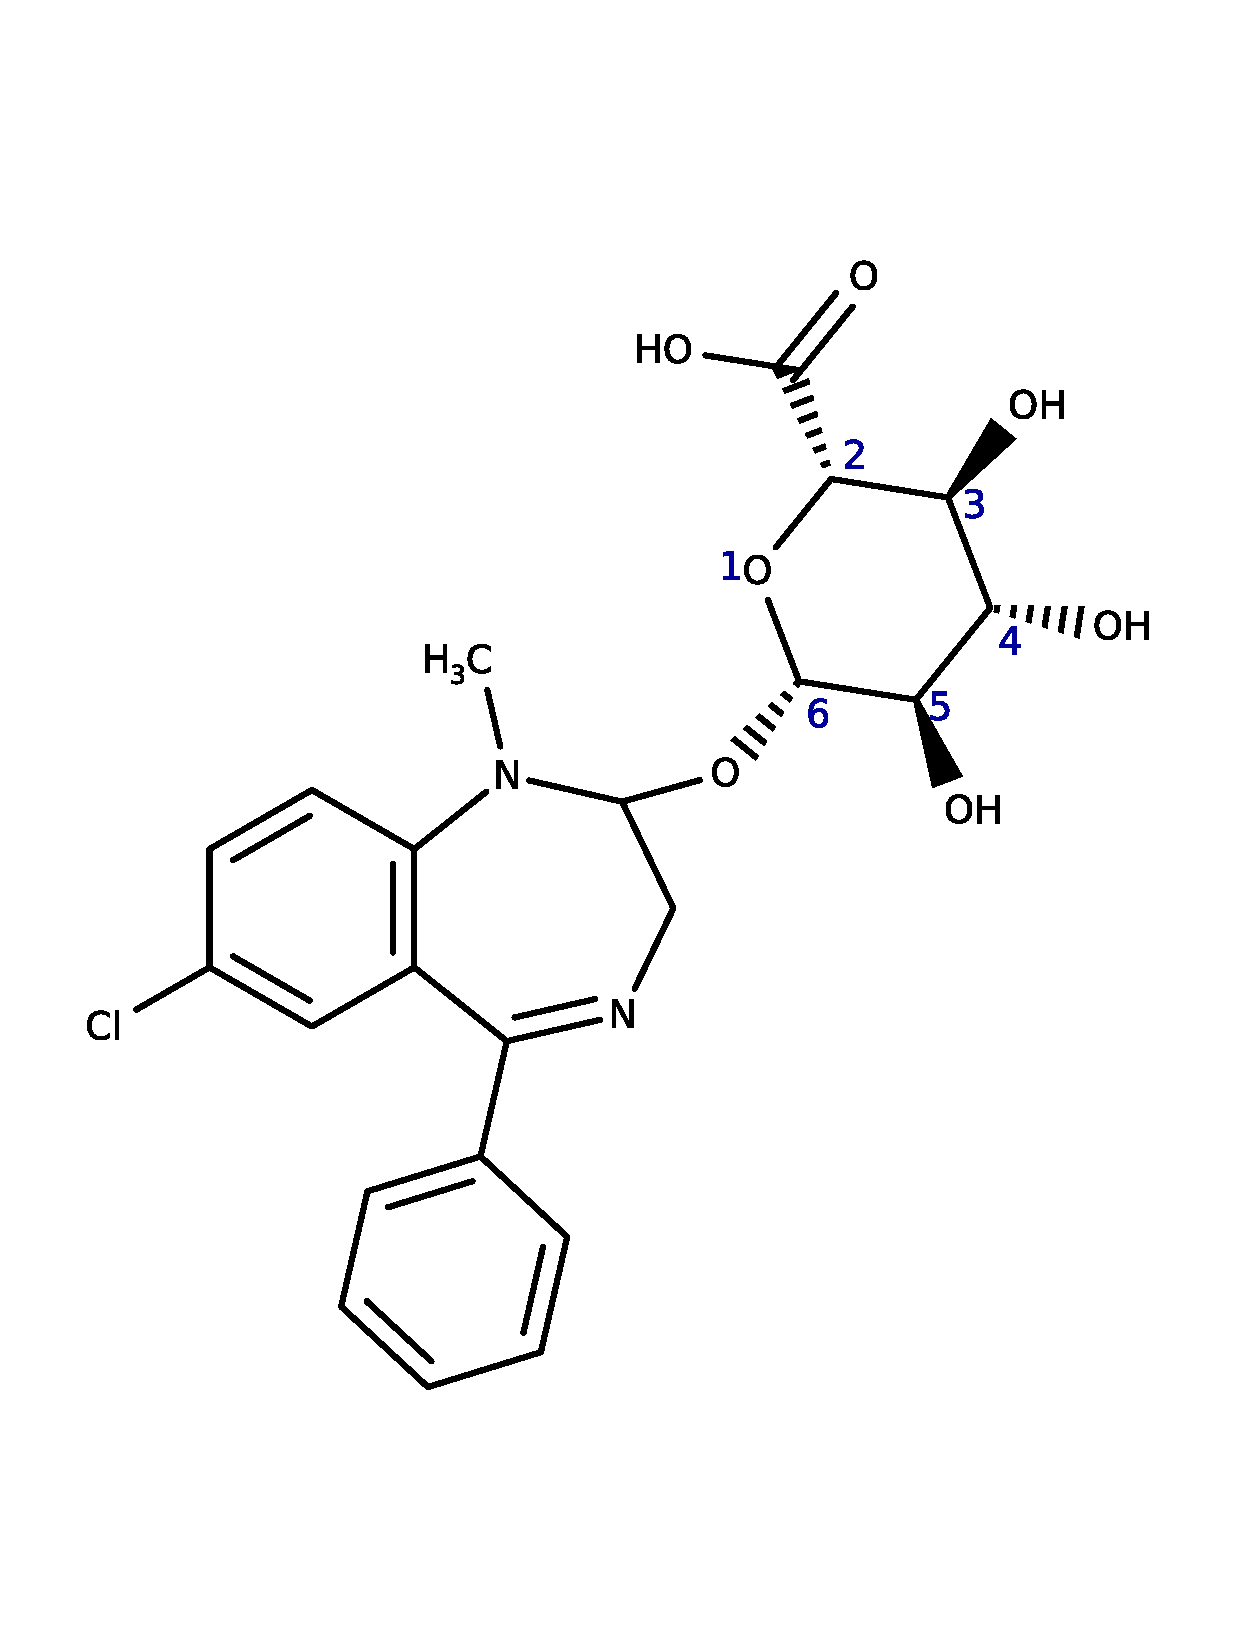
\includegraphics[width=\linewidth]{glucu.pdf}
		\captionof{figure}{Nordiazepam O-glucuronide}
		\label{fig:norgluc}
	\end{minipage}
\end{figure}





\section{Lorazepam} 
%The structure of the 3-0-phenolic glucuronie
Lorazepam is hepatically metabolized by conjugation to the 3-0-phenolic glucuronide which gives Lorazepam glucuronide \emph{Fig} \ref{fig:lorgluc}.\cite{elliott1976metabolism}

\begin{figure}[h]
	\centering
	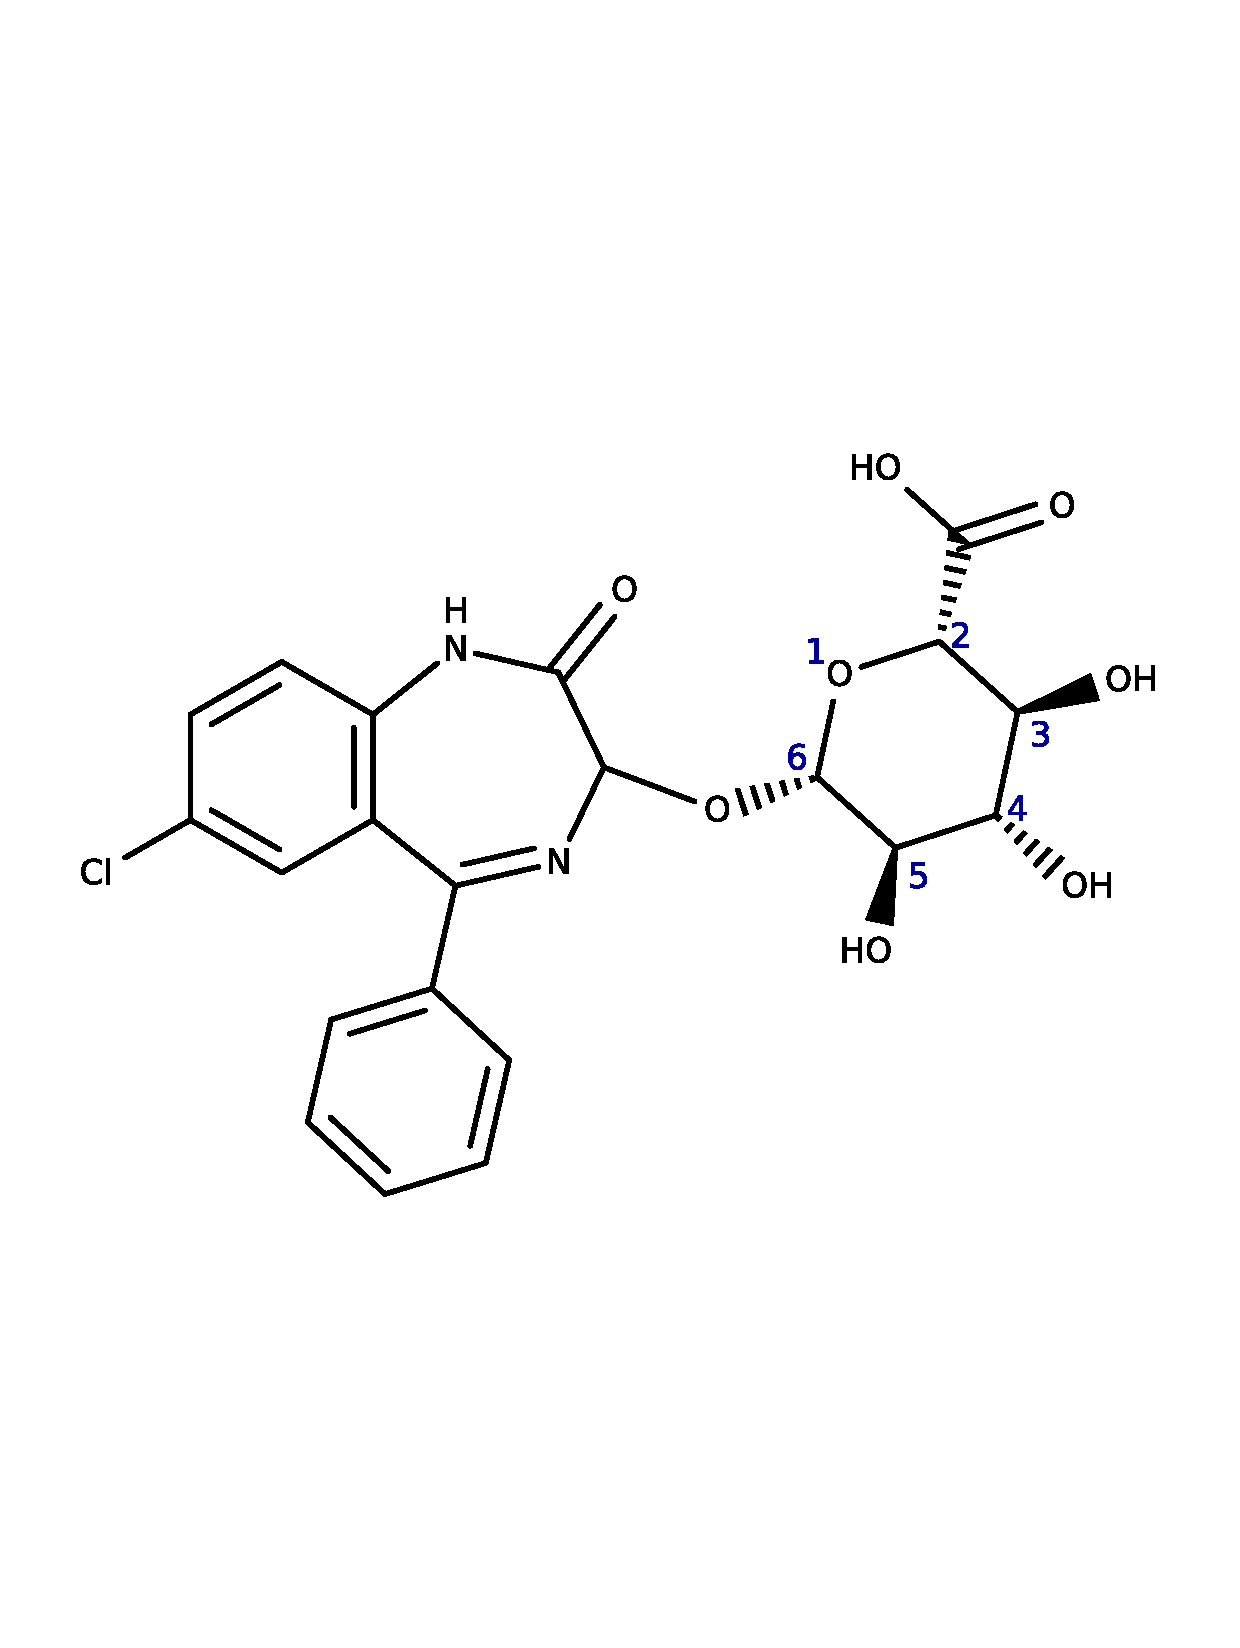
\includegraphics[width=\textwidth]{lorazapamglucu.pdf}
	\captionof{figure}{Nordiazepam O-glucuronide}
	\label{fig:lorgluc}
\end{figure}

%Active Metabolites
\input{parts/acmetab.tex}
%Side Effects
\chapter{Side Effects}
\section{Chlordiazepoxide}

\section{Diazepam}
The most common side effects are drowsiness, fatigue, ataxia\footnote{the loss of full control of bodily movements.
}, and muscle weakness.

The following symptoms are minor, but still reported.
\subsubsection{Central Nervous System} confusion, depression, dysarthria, headache, slurred speech, tremor, vertigo

\subsubsection{Gastrointestinal System} constipation, nausea, gastrointestinal disturbances

\section{Lorazepam} 
Side effects of Lorazepam include
\begin{itemize}
\item Drowsiness
\item Dizziness
\item Tiredness
\item Muscle weakness
\item Headache
\item Blurred vision
\item Sleep problems (insomnia)
\item Loss of balance or coordination
\item Forgetfulness or amnesia
\item Difficulty concentrating
\item Nausea
\item Vomiting
\item Constipation
\item Changes in appetite
\item Skin rash
\end{itemize}
Serious side effects. If any of these is present, seek medical attention immediately
\begin{itemize}
\item confusion, depressed mood, thoughts of suicide or hurting yourself.
\item hyperactivity, agitation, hostility.
\item hallucinations.
\item feeling light-headed, fainting.
\end{itemize}
%Toxicity done
\chapter{Toxicity}
\section{Chlordiazepoxide}
LD$_{50}$\footnote{lethal dose in 50\% of the subjects}=537 mg/kg (Orally in rats). Symptoms of overdose include respiratory depression, muscle weakness, somnolence (general depressed activity).



\section{Diazepam}
Signs of overdose include somnolence\footnote{drowsiness}, confusion, coma, and diminished reflexes. Respiration, pulse and blood pressure should be monitored.


\section{Lorazepam} 
Respiratory depression is the most adverse event caused by lorazepam. LD$_{50, mouse}$, oral = 1850 mg/kg.

%Dosage forms done
\chapter{Dosage Forms}

\section{Chlordiazepoxide}
Chlordiazepoxide is exclusively present as capsules with strengths of (5 mg - 10 mg - 25 mg)

Generics are present as either Chlordiaze-poxide HCL or Chlordiazepoxide Hydrychloride as capsules or gelatin coated capsules with strengths of (5 mg - 10 mg - 25 mg)


\section{Diazepam}
Diazepam is present as an injection for intramuscular route with strength of about (5 mg/mL). Liquid and Emulsions are also present for intramuscular;intravenous routes with strengths of (5 mg - 10 mg). Oral doses are mostly present as tablets with strengths of (2 mg - 5 mg - 10 mg). Gels are present for rectal route with strengths of (10 mg/2mL - 5 mg - 20 mg/4mL - 2.5 mg/0.5mL)

\section{Lorazepam} 
Lorazepam is present as oral, sublingual, intramuscular, and intravenous dosage forms. 


The oral along with the sublingual forms are present as tablets with strengths of(0.5 mg- 1 mg - 2 mg). A concentrated solution of 2 mg of Lorazepam is also present for oral route.

Solutions and liquid are present for intramuscular;intravenous route with strengths of (2 mg/mL - 4 mg/mL)

The most abundant form of generics is the tablet form for oral route of strength (1 mg/1). Liquids and solutions for intramuscular;intravenous routes are present with concentrations 2mg/mL.


\bibliographystyle{ieeetr}
\bibliography{sample} 
\end{document}


